\section{Resultate}
\label{sec:resultate}

\subsection{Beispiel mit farbig hervorgehobener Tabelle}
\label{subsec:beispiel-farbtabelle}
Mit dem Paket \texttt{xcolor} (Option \texttt{table}) können einzelne Tabellenzeilen
hervorgehoben werden, siehe Tabelle~\ref{tab:beispiel-farbtabelle}.

\begin{table}[h!]
    \centering
    \caption{Beispieltabelle mit farbig hervorgehobenen Zeilen.}
    \label{tab:beispiel-farbtabelle}
    \begin{tabularx}{\textwidth}{l *{2}{>{\centering\arraybackslash}X}}
        \toprule
        \textbf{Punktnr.} & \textbf{Abweichung [cm]} & \textbf{Bemerkung} \\
        \midrule
        1001 & 1.2 & Platzhalter \\
        \rowcolor{lightgray}
        1002 & 3.4 & \textcolor{red}{\textbf{Auffälliger Wert}} \\
        1003 & 0.8 & Platzhalter \\
        \bottomrule
    \end{tabularx}
\end{table}

\subsection{Beispiel einer mehrspaltigen Liste}
\label{subsec:beispiel-multicol}
Mit dem Paket \texttt{multicol} können Aufzählungen auf mehrere Spalten verteilt werden,
zum Beispiel für Listen mit vielen kurzen Einträgen: \todo{Dies ist ein To-do Kommentar}

\begin{multicols}{2}
    \begin{itemize}
        \item Eintrag 1
        \item Eintrag 2
        \item Eintrag 3
        \item Eintrag 4
        \item Eintrag 5
        \item Eintrag 6
    \end{itemize}
\end{multicols}

\subsection{Beispiel eines einfachen Diagramms}
\label{subsec:beispiel-tikz}
Mit dem Paket \texttt{tikz} können einfache Diagramme direkt in \LaTeX{} erstellt werden,
siehe \Cref{fig:beispiel-tikz}.

\begin{figure}[h!]
    \centering
    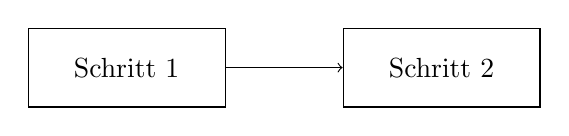
\begin{tikzpicture}
        \node[draw, rectangle, minimum width=2.5cm, minimum height=1cm] (a) at (0,0) {Schritt 1};
        \node[draw, rectangle, minimum width=2.5cm, minimum height=1cm] (b) at (4,0) {Schritt 2};
        \draw[->] (a) -- (b);
    \end{tikzpicture}
    \caption{Beispiel für ein einfaches \texttt{tikz}-Diagramm.}
    \label{fig:beispiel-tikz}
\end{figure}

\FloatBarrier